\chapter{Historischer Kontext der BRD-Wirtschaftsgeschichte}

\section{Einführung: Deutschlands besonderer Weg}

Die wirtschaftliche Entwicklung der Bundesrepublik Deutschland von 1960 bis 2023 ist geprägt von außergewöhnlichen Erfolgen, tiefen Krisen und fundamentalen Transformationen. Dieser Zeitraum umfasst nicht nur sechs Jahrzehnte wirtschaftlicher Dynamik, sondern auch politische Systemwechsel, geopolitische Umwälzungen und tiefgreifende gesellschaftliche Veränderungen.

\section{Die Ausgangslage 1960}

\subsection{Wirtschaftliche Situation}
\begin{itemize}
\item \textbf{BIP pro Kopf}: 13.000 DM (ca. 6.500€ in heutiger Kaufkraft)
\item \textbf{Arbeitslosigkeit}: 1,3\% (Vollbeschäftigung)
\item \textbf{Industrieanteil}: 45\% des BIP
\item \textbf{Exportquote}: 15\% des BIP
\item \textbf{Währungsreserven}: 30 Mrd. DM
\end{itemize}

\subsection{Soziale Struktur}
\begin{itemize}
\item \textbf{Bevölkerung}: 55 Millionen (Westdeutschland)
\item \textbf{Gastarbeiter}: Erste Anwerbeabkommen mit Italien (1955), Spanien, Griechenland
\item \textbf{Lohnquote}: 72\% (Anteil der Arbeitnehmerentgelte am Volkseinkommen)
\item \textbf{Rentenalter}: 65 Jahre, durchschnittliche Lebenserwartung: 67 Jahre (Männer)
\end{itemize}

\subsection{Institutioneller Rahmen}
\begin{itemize}
\item \textbf{Soziale Marktwirtschaft}: Ludwig Erhards Konzept in der Praxis
\item \textbf{Bundesbank}: Seit 1957 unabhängige Währungshüterin
\item \textbf{EGKS/EWG}: Beginn der europäischen Integration
\item \textbf{Bretton Woods}: Feste Wechselkurse, Dollar-Gold-Standard
\end{itemize}

\section{Periodisierung der BRD-Wirtschaftsgeschichte}

\subsection{Traditionelle Periodisierung}
\begin{table}[ht]
\centering
\begin{tabular}{lll}
\toprule
\textbf{Periode} & \textbf{Charakterisierung} & \textbf{Schlüsselereignisse} \\
\midrule
1960--1973 & Wirtschaftswunder & Vollbeschäftigung, Wachstum \\
1974--1982 & Stagflation & Ölkrisen, Arbeitslosigkeit \\
1983--1990 & Konsolidierung & Neue Sachlichkeit, EG-Integration \\
1991--2005 & Vereinigungszeit & Aufbau Ost, Euro-Einführung \\
2006--2019 & Exportweltmeister & Agenda 2010, Finanzkrise, Eurokrise \\
2020--2023 & Multikrise & Pandemie, Energiekrise, Inflation \\
\bottomrule
\end{tabular}
\caption{Traditionelle wirtschaftshistorische Periodisierung}
\label{tab:periodisierung-traditionell}
\end{table}

\subsection{Neue Periodisierung nach GWI-D}
\begin{table}[ht]
\centering
\begin{tabular}{lll}
\toprule
\textbf{Periode} & \textbf{GWI-D-Charakter} & \textbf{Dominante Entwicklung} \\
\midrule
1960--1973 & Inklusives Wachstum & Wirtschaft + Gerechtigkeit steigen \\
1974--1982 & Erste Spaltung & Wirtschaft stagniert, Gerechtigkeit sinkt \\
1983--1998 & Konsolidierung & Wirtschaft erholt, Zusammenhalt schwindet \\
1999--2008 & Exportfixierung & Wirtschaft wächst, Verteilung verschlechtert \\
2009--2020 & Krisenbewältigung & Zusammenhalt stärkt sich trotz Schocks \\
2021--2023 & Neue Spaltung & Alle Säulen unter Druck \\
\bottomrule
\end{tabular}
\caption{Periodisierung nach GWI-D-Perspektive}
\label{tab:periodisierung-gwid}
\end{table}

\section{Strukturwandel im Zeitverlauf}

\subsection{Sektoraler Wandel}
\begin{figure}[ht]
\centering
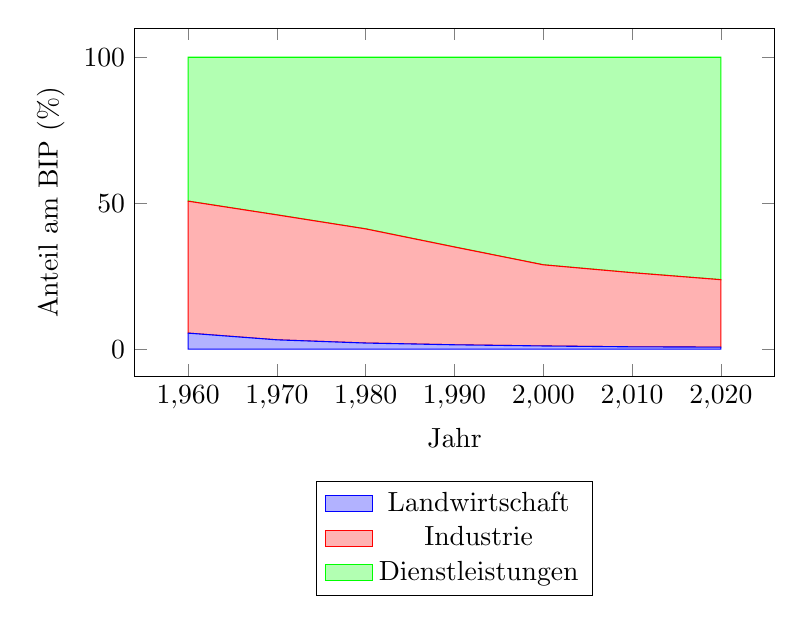
\begin{tikzpicture}
\begin{axis}[
    width=0.8\textwidth,
    height=6cm,
    ylabel={Anteil am BIP (\%)},
    xlabel={Jahr},
    xtick={1960,1970,1980,1990,2000,2010,2020},
    legend style={at={(0.5,-0.3)},anchor=north},
    stack plots=y,
    area style,
]
\addplot+[blue, fill=blue!30] table {
Jahr Landwirtschaft
1960 5.5
1970 3.2
1980 2.1
1990 1.5
2000 1.1
2010 0.8
2020 0.7
} \closedcycle;
\addplot+[red, fill=red!30] table {
Jahr Industrie
1960 45.2
1970 42.8
1980 39.1
1990 33.5
2000 27.8
2010 25.4
2020 23.1
} \closedcycle;
\addplot+[green, fill=green!30] table {
Jahr Dienstleistungen
1960 49.3
1970 54.0
1980 58.8
1990 65.0
2000 71.1
2010 73.8
2020 76.2
} \closedcycle;
\legend{Landwirtschaft, Industrie, Dienstleistungen}
\end{axis}
\end{tikzpicture}
\caption{Sektoraler Wandel der deutschen Wirtschaft 1960--2020}
\label{fig:sektoraler-wandel}
\end{figure}

\subsection{Demografische Entwicklung}
\begin{itemize}
\item \textbf{Bevölkerungswachstum}: 55 Mio. (1960) → 84 Mio. (2023)
\item \textbf{Altersstruktur}: Medianalter von 34 auf 47 Jahre gestiegen
\item \textbf{Erwerbsquote}: Von 45\% auf 58\% gestiegen (vor allem durch Frauenerwerbstätigkeit)
\item \textbf{Migration}: Nettomigration von durchschnittlich 200.000 pro Jahr
\end{itemize}

\section{Institutionelle Rahmenbedingungen}

\subsection{Währungsordnungen}
\begin{enumerate}
\item \textbf{1960--1973}: Bretton-Woods-System (feste Wechselkurse)
\item \textbf{1973--1999}: Floating D-Mark (starke Aufwertung)
\item \textbf{1999--heute}: Euro (zunächst unterbewertet, dann überbewertet)
\end{enumerate}

\subsection{Arbeitsbeziehungen}
\begin{itemize}
\item \textbf{1960er}: Starke Gewerkschaften, hohe Tarifbindung (85\%)
\item \textbf{1980er}: Beginn der Erosion, erste Öffnungsklauseln
\item \textbf{2000er}: Agenda 2010, Hartz-Reformen, Flexibilisierung
\item \textbf{2020er}: Mindestlohn, Renaissance der Tarifbindung?
\end{itemize}

\subsection{Sozialstaat}
\begin{table}[ht]
\centering
\begin{tabular}{lccc}
\toprule
\textbf{Jahr} & \textbf{Sozialquote (\%)} & \textbf{Rentenniveau (\%)} & \textbf{Arbeitslosenquote (\%)} \\
\midrule
1960 & 22,1 & 55 & 1,3 \\
1975 & 32,5 & 60 & 4,7 \\
1990 & 29,8 & 55 & 7,2 \\
2005 & 30,5 & 53 & 11,7 \\
2020 & 33,5 & 48 & 5,9 \\
2023 & 34,2 & 48 & 5,7 \\
\bottomrule
\end{tabular}
\caption{Entwicklung des Sozialstaats}
\label{tab:sozialstaat-entwicklung}
\end{table}

\section{Externe Schocks und Krisen}

\subsection{Ölkrisen (1973, 1979)}
\begin{itemize}
\item \textbf{Auslöser}: Jom-Kippur-Krieg, Iranische Revolution
\item \textbf{Wirkung}: Ölpreis vervierfacht sich
\item \textbf{Folgen}: Stagflation, Ende des Wirtschaftswunders
\item \textbf{Antwort}: Energiesparen, Diversifizierung
\end{itemize}

\subsection{Wiedervereinigung (1990)}
\begin{itemize}
\item \textbf{Wirtschaftlicher Schock}: Produktivitätsgefälle 1:3
\item \textbf{Kosten}: 2 Billionen € Transferleistungen
\item \textbf{Chancen}: Binnenmarktverdopplung, Fachkräfte
\item \textbf{Langfristige Wirkung}: Noch heute Produktivitätsrückstand Ost: 80\% des Westniveaus
\end{itemize}

\subsection{Finanzkrise (2008/09)}
\begin{itemize}
\item \textbf{Ursprung}: US-Subprime-Krise
\item \textbf{Auswirkung auf Deutschland}: Exporteinbruch -15\%
\item \textbf{Policy-Response}: Konjunkturpakete, Kurzarbeitergeld
\item \textbf{Paradox}: Soziale Absicherung milderte Krisenfolgen
\end{itemize}

\subsection{Eurokrise (2010--2015)}
\begin{itemize}
\item \textbf{Deutsche Rolle}: Gläubiger, Reformbefürworter
\item \textbf{Wirtschaftliche Wirkung}: Gefahr für Exportmärkte
\item \textbf{Innere Spannungen}: Nord-Süd-Konflikt in Europa
\item \textbf{Langfristig}: Vertiefung der EU, Fiskalunion
\end{itemize}

\subsection{Pandemie (2020/21)}
\begin{itemize}
\item \textbf{Wirtschaftlicher Einbruch}: -5,7\% BIP (2020)
\item \textbf{Staatliche Antwort}: 400 Mrd. € Hilfspakete
\item \textbf{Soziale Wirkung}: Kurzarbeit statt Massenarbeitslosigkeit
\item \textbf{Strukturell}: Digitalisierungsschub, Homeoffice
\end{itemize}

\subsection{Energiekrise (2022)}
\begin{itemize}
\item \textbf{Auslöser}: Ukraine-Krieg, Sanktionen
\item \textbf{Preiseffekte}: Gas +500\%, Strom +300\%
\item \textbf{Wirtschaftlich}: Gefahr der Deindustrialisierung
\item \textbf{Politisch}: Beschleunigung der Energiewende
\end{itemize}

\section{Deutschland im internationalen Vergleich}

\subsection{Wachstumsperformance}
\begin{itemize}
\item \textbf{1960--1973}: Überdurchschnittlich (+4,2\% p.a. vs. OECD: +3,8\%)
\item \textbf{1974--2000}: Durchschnittlich (+2,1\% vs. OECD: +2,2\%)
\item \textbf{2001--2019}: Unterdurchschnittlich (+1,2\% vs. OECD: +1,8\%)
\item \textbf{Gesamt 1960--2023}: +2,4\% p.a. (OECD: +2,6\%)
\end{itemize}

\subsection{Produktivitätsentwicklung}
\begin{itemize}
\item \textbf{Arbeitsproduktivität}: Über OECD-Durchschnitt
\item \textbf{Total Factor Productivity}: Seit 2000 stagnierend
\item \textbf{Innovationsfähigkeit}: Stark in traditioneller Industrie, schwach in Digitalisierung
\end{itemize}

\subsection{Außenhandel}
\begin{table}[h]
\centering
\begin{tabular}{lccc}
\toprule
\textbf{Jahr} & \textbf{Exportquote (\%)} & \textbf{Handelsbilanz (\% BIP)} & \textbf{Top-Exportgüter} \\
\midrule
1960 & 15,2 & +1,2 & Maschinen, Chemie \\
1980 & 23,8 & +2,1 & Autos, Maschinen \\
2000 & 33,5 & +1,8 & Autos, Maschinen, Chemie \\
2020 & 47,1 & +7,5 & Autos, Maschinen, Pharma \\
2023 & 44,8 & +6,2 & Autos, Maschinen, Chemie \\
\bottomrule
\end{tabular}
\caption{Entwicklung des deutschen Außenhandels}
\label{tab:aussenhandel}
\end{table}

\section{Politische Weichenstellungen}

\subsection{Große Reformpakete}
\begin{enumerate}
\item \textbf{Stabilitätsgesetz (1967)}: Konjunktursteuerung, Globalsteuerung
\item \textbf{Ökosteuer (1999)}: Ökologische Steuerreform
\item \textbf{Agenda 2010 (2003--2005)}: Arbeitsmarktreformen, Hartz-Gesetze
\item \textbf{Energiewende (2011)}: Atomausstieg nach Fukushima
\item \textbf{Zeitenwende (2022)}: Aufrüstung, Energieunabhängigkeit
\end{enumerate}

\subsection{Steuerpolitik}
\begin{itemize}
\item \textbf{Spitzensteuersatz}: Von 53\% (1960) auf 42\% (2023) gesenkt
\item \textbf{Körperschaftssteuer}: Von 56\% auf 15\% gesenkt
\item \textbf{Mehrwertsteuer}: Von 10\% auf 19\% erhöht
\item \textbf{Steuerquote}: Relativ konstant bei 23--25\% des BIP
\end{itemize}

\section{Gesellschaftlicher Wandel}

\subsection{Wertewandel}
\begin{itemize}
\item \textbf{1960er}: Materialistische Werte (Sicherheit, Ordnung)
\item \textbf{1980er}: Postmaterialismus (Selbstverwirklichung, Umwelt)
\item \textbf{2000er}: Individualisierung, Flexibilisierung
\item \textbf{2020er}: Sicherheitsbedürfnis, Nachhaltigkeit
\end{itemize}

\subsection{Soziale Mobilität}
\begin{itemize}
\item \textbf{1960--1980}: Aufstiegsgesellschaft (Bildungsexpansion)
\item \textbf{1980--2000}: Verlangsamung der Mobilität
\item \textbf{2000--2020}: Zunahme der Persistenz (Vererbung von Status)
\end{itemize}

\section{Zusammenfassung: Deutschlands wirtschaftshistorische Besonderheiten}

\subsection{Erfolgsfaktoren}
\begin{enumerate}
\item \textbf{Institutionelle Stabilität}: Unabhängige Bundesbank, stabile Demokratie
\item \textbf{Mittelständische Struktur}: Hidden Champions, industrielles Rückgrat
\item \textbf{Exportorientierung}: Hochwertige Produkte, globale Nachfrage
\item \textbf{Sozialpartnerschaft}: Kooperative Arbeitsbeziehungen (bis 1990er)
\item \textbf{Bildungssystem}: Duale Ausbildung, Fachkräfte
\end{enumerate}

\subsection{Strukturelle Schwächen}
\begin{enumerate}
\item \textbf{Demografie}: Alternde Gesellschaft, Fachkräftemangel
\item \textbf{Digitalisierung}: Langsame Adaption, fehlende Plattformen
\item \textbf{Infrastruktur}: Investitionsstau, Sanierungsbedarf
\item \textbf{Bürokratie}: Regulierungsdichte, langsame Verfahren
\item \textbf{Energieabhängigkeit}: Historisch von Importen abhängig
\end{enumerate}

\subsection{Deutschland im europäischen Kontext}
\begin{itemize}
\item \textbf{Wirtschaftsmotor}: Größte Volkswirtschaft der EU
\item \textbf{Stabilitätsanker}: Politisch und wirtschaftlich
\item \textbf{Zahlmeister}: Nettozahler in EU-Haushalt
\item \textbf{Reformmodell}: Agenda 2010 als Vorbild für Südeuropa
\item \textbf{Spannungsfeld}: Nationale Interessen vs. europäische Solidarität
\end{itemize}

\section{Ausblick auf die GWI-D-Analyse}

Der historische Kontext bildet das Fundament für die folgende empirische Analyse. Vor dem Hintergrund dieser wirtschaftlichen, sozialen und politischen Entwicklungen wird der GWI-D zeigen:

\begin{enumerate}
\item Wie sich die vier Säulen des Gemeinwohls im Zeitverlauf entwickelt haben
\item Welche Perioden tatsächlich ganzheitlichen Fortschritt brachten
\item Wie Krisen und Reformen auf die verschiedenen Dimensionen wirkten
\item Wo Deutschland heute steht – und welche Lehren sich für die Zukunft ziehen lassen
\end{enumerate}

Die historische Betrachtung macht deutlich: Wirtschaftliche Entwicklung ist nie eindimensional. Der GWI-D hilft, diese Mehrdimensionalität systematisch zu erfassen und zu bewerten.